%% LyX 2.0.4 created this file.  For more info, see http://www.lyx.org/.
%% Do not edit unless you really know what you are doing.
\documentclass[oneside,dutch]{amsart}
\usepackage[T1]{fontenc}
\usepackage[latin9]{inputenc}
\usepackage[a4paper]{geometry}
\geometry{verbose,tmargin=3cm,bmargin=3cm,lmargin=2cm,rmargin=2cm}
\setlength{\parskip}{\smallskipamount}
\setlength{\parindent}{0pt}
\usepackage{amsthm}
\usepackage{graphicx}
\graphicspath{{Figures/}}

\makeatletter
%%%%%%%%%%%%%%%%%%%%%%%%%%%%%% Textclass specific LaTeX commands.
\numberwithin{equation}{section}
\numberwithin{figure}{section}

\makeatother

\usepackage{babel}
\begin{document}

\title{Data verwerking zonder periodieke afhankelijkheid}


\author{N.G. Schultheiss}

\maketitle

\section{Inleiding}

Deze module volgt op de module ``Data verwerking met periodieke afhankelijkheid'',
waarin werd uitgelegd hoe je een spreadsheet met gegevens van de detectoren
kunt maken. Hier werd uitgelegd hoe conclusies te trekken zijn, als
er sprake is van een periodieke afhankelijkheid. In het geval van
de afhankelijkheid van weersverschijnselen zoals bliksem, zal dit
niet periodiek zijn. Het is namelijk niet zo dat er om een bepaalde
tijd een bliksemflits wordt gegenereerd. 


\section{Kansen}

Om iets over de afhankelijkheid van een verschijnsel te kunnen zeggen,
bekijken we eerst de kans (probability: \emph{P}()) dat het verschijnsel
heeft plaatsgevonden. Een dergelijk grafiek is te zien in figuur 2.1.

\begin{figure}[h]
\noindent \begin{centering}
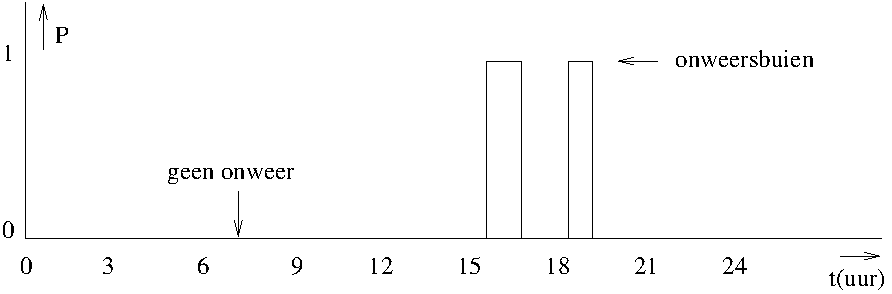
\includegraphics[scale=0.75]{buien}
\par\end{centering}

\caption{De kans op onweer}
\end{figure}


We moeten eigenlijk twee kansen vergelijken, de kans dat er onweer
is en de kans dat er geen onweer is. De kans dat er geen onweer is,
is te zien in figuur 2.2.

\begin{figure}[h]
\noindent \begin{centering}
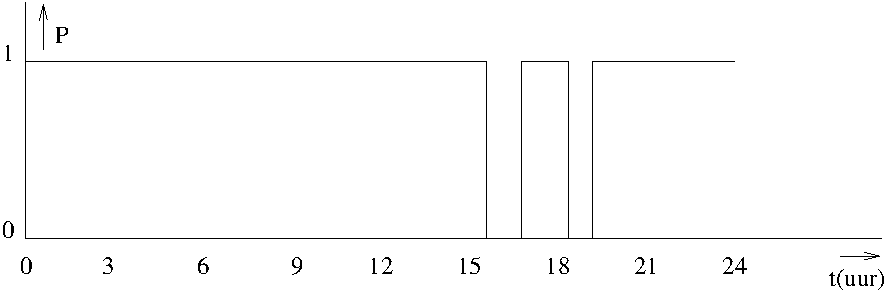
\includegraphics[scale=0.75]{geenBuien}
\par\end{centering}

\caption{De kans dat er geen onweer is.}
\end{figure}



\paragraph*{Opdracht 1:}

\emph{Leg uit dat op ieder tijdstip geldt: P}(onweer)+\emph{P}(geenOnweer)=1\emph{.}

Laten we eerst aannemen dat de kosmische straling niet afhangt van
het weer. In grafiek 2.3 is de kosmische straling daarom constant
genomen. Om te kijken of de kosmische straling nu afhangt van het
onweer, vermenigvuldigen we op alle tijdstippen de kans op onweer
met het aantal co�ncidenties. Als we alle de uitkomsten voor de hele
dag optellen krijgen we een getal. Hetzelfde is te doen met de kans
dat er geen onweer is. Nu krijgen we weer een getal. Als we deze getallen
vergelijken, lijkt het of de kans op kosmische straling bij mooi weer
groter is. 

\begin{figure}[h]
\noindent \begin{centering}
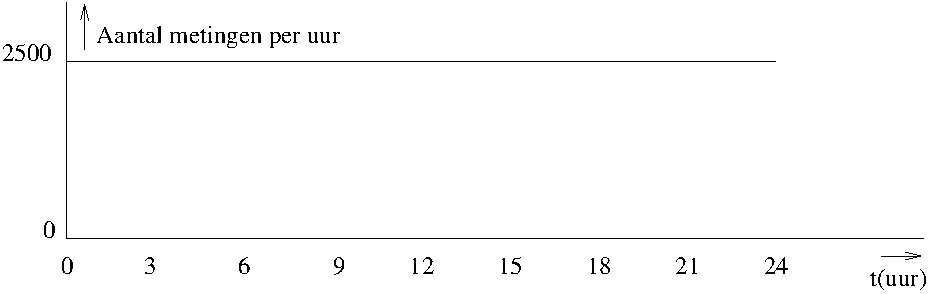
\includegraphics[scale=0.75]{onafhankelijk}
\par\end{centering}

\caption{Constante kosmische straling}
\end{figure}



\paragraph*{Opdracht 2:}

\emph{Toon aan dat dit resultaat te corrigeren is door in beide gevallen
te delen door het oppervlak onder de kans-grafieken. }


\section{Een procedure voor een spreadsheet}

We kunnen dit op de volgende manier in een spreadsheet verwerken:
\begin{itemize}
\item Laad een .csv bestand van ``http://data.hisparc.nl'' in een spreadsheetprogramma.
\item Bereken de kans voor ieder uur dat er onweer was en zet deze waarden
in een ``onweerkolom''. Is er in een uur een kwartier onweer geweest,
dan geldt: \emph{P}(onweer)=0,25 (of 0.25 als het spreadsheetprogramma
niet in het nederlands is ge�nstalleerd). 
\item De kans dat er in dit geval geen onweer is, is te berekenen met: \emph{P}(geenOnweer)=1-\emph{P}(onweer).
Deze waarden staan in de kolom ``geenOnweer''.
\item Bereken de som voor de kolommen ``onweer'' en ``geenOnweer''.
\item Bereken op ieder tijdstip \emph{aantalCo�ncidenties}{*}\emph{P}(onweer)
en \emph{aantalCo�ncidenties}{*}\emph{P}(geenOnweer) en zet deze waarden
in twee kolommen.
\item Bereken de som van \emph{aantalCo�ncidenties}{*}\emph{P}(onweer) en
deel dit door de som van de kolom ``onweer'', dit is ``deKansOpOnweer''. 
\item Bereken de som van \emph{aantalCo�ncidenties}{*}\emph{P}(geenOnweer)
en deel dit door de som van de kolom ``geenOnweer'', dit is ``geenKansOpOnweer''. 
\item We kunnen nu ``deKansOpOnweer'' en ``geenKansOpOnweer'' vergelijken.
De grootste wint.
\end{itemize}
\begin{figure}[h]
\noindent \begin{centering}
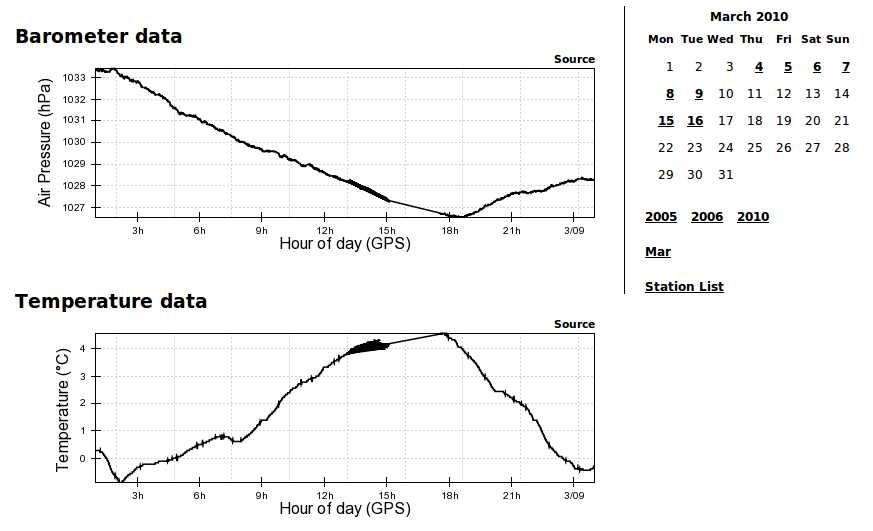
\includegraphics[width=16cm]{Screenshot}
\par\end{centering}

\caption{De weerdata voor 8 maart 2010}
\end{figure}


Met deze aanpak zijn er veel soortgelijke problemen op te lossen.
We kunnen bijvoorbeeld kijken of er een hemellichaam boven de detector
is. Op een vergelijkbare wijze is een grafiek te maken met de kans
dat een hemellichaam boven de detector is en de kans dat dit hemellichaam
niet boven de detector is.


\paragraph*{Opdracht 3:}

\emph{Station 98 geeft de Nikhef weerinformatie, deze is te zien in
figuur 3.1. Op het Nikhef zijn ook diverse detectoren van kosmische
straling te vinden. Leg uit wat het probleem is, als we willen onderzoeken
of de kosmische straling van de luchtdruk afhangt.}

Als we op ``source'' klikken kunnen we hier ook een .csv bestand
downloaden. Dit bestand werkt met een tijdstempel: het aantal seconden
vanaf 1 januari 1970. Aangezien een uur 3600s heeft, kunnen we hier
ook een tabel met de weergegevens per minuut / uur van maken. 


\section{Correlatie van twee grafieken}

Als we twee grafieken willen correleren, moeten we dit iets slimmer
aanpakken. We gaan uit van de luchtdrukafhankelijk van de kosmische
straling.
\begin{itemize}
\item Haal de gegevens van de kosmische straling op en zet deze in een spreadsheet.
\item Haal de gegevens van het weer op en zet deze in een spreadsheet.
\item Bepaal het gemiddelde van de luchtdruk over de dag.
\item Bepaal hoeveel de luchtdruk op ieder moment afwijkt van het gemiddelde
en zet deze waarden in een nieuwe kolom.
\item Vermenigvuldig de afwijking met de kosmische straling en zet dit resultaat
in een extra kolom.
\item Tel alle waarden van de extra kolom op. Is het resultaat positief
dan geeft een hogere luchtdruk meer kosmische straling. Is het resultaat
negatief dan geeft een lagere luchtdruk meer kosmische straling.
\end{itemize}

\paragraph*{Opdracht 4:}

\emph{Vergelijk de procedure hierboven met de procedure uit hoofdstuk
3. Toon aan dat de procedure van hoofdstuk 4 hetzelfde resultaat geeft
als de procedure uit hoofdstuk 4.}
\end{document}
